%\documentclass[wsdraft]{ws-procs11x85}

\documentclass{ws-procs11x85}
\usepackage{ws-procs-thm}           % comment this line when `amsthm / theorem / ntheorem` package is used
\usepackage{algorithmic}

\begin{document}

\title{Improving QSAR Modeling for Predictive Toxicology using Publicly Aggregated Semantic Graph Data and Graph Neural Networks}

\author{Joseph~D.~Romano$^*$, Yun~Hao$^*$, and Jason~H.~Moore$^\dag$}

\address{Institute for Biomedical Informatics, University of Pennsylvania,\\
Philadelphia, Pennsylvania 19104, United States\\
$^\dag$Corresponding author e-mail: jhmoore@upenn.edu\\
$^*$These authors contributed equally.}

\begin{abstract}
Quantitative Structure-Activity Relationship (QSAR) modeling is the most common computational technique for predicting toxicity for specific chemicals, but a lack of methodological innovations have led to underwhelming performance of QSAR in modern applications.
We show that contemporary QSAR modeling for predictive toxicology can be substantially improved by incorporating semantic graph data aggregated from open-access public databases, and analyzing those data in the context of graph neural networks (GNNs).
Furthermore, we introspect the GNNs to demonstrate how they can lead to more interpretable applications of QSAR, and use ablation analysis to explore the contribution of different data elements to the final models' performance.
\end{abstract}

\keywords{Toxicology; Graph neural networks; Data aggregation; QSAR; Artificial intelligence.}

\section{Introduction}\label{introduction}
Evaluating the toxicity of chemicals is an essential component of pharmaceutical and environmental research.
Traditionally, the task of establishing toxicity has been accomplished using \textit{in vivo} models, where a model organism is exposed to a chemical of interest and observed for toxic effects, or by performing retrospective observational studies on human populations in the context of epidemiological analyses.
Both of these approaches are costly and time consuming, and given the hundreds of thousands of compounds of toxicological interest, innovative alternatives are needed to rapidly screen chemicals.
In recent decades, predictive toxicology and large-scale chemical screening efforts have emerged to address this issue.

Quantitative Structure-Activity Relationship (QSAR) modeling is arguably the most common method for predicting \textit{in silico} whether a chemical will cause a toxic response.
Briefly, QSAR modeling involves collecting quantitative descriptions of molecular structures, and then fitting a statistical model (e.g., logistic regression, or other supervised machine learning algorithms) to chemicals where a toxic endpoint of interest is already known.
Since each data point used to train a model is itself the outcome of a single experiment, QSAR is a meta-analysis approach that is complicated not only by the challenge of capturing relevant structural features of chemicals, but also by errors, biases, and ambiguities in the underlying experiments used to generate the training data.
Consequently, QSAR is heavily criticized for its disappointing performance on many tasks.
The computational toxicology community has long acknowledged the need for new methodological innovations to improve QSAR performance, but few have emerged in the past several decades.

In this study, we address these issues by augmenting the traditional QSAR approach with multimodal graph data aggregated from several public data sources, and analyzing those data in the context of a heterogeneous graph convolutional neural network (GCNN) model.
We evaluate the model using 59 assays and their accompanying chemical screening data from the Tox21 data repository, and compare its performance to two rigorously defined traditional QSAR models consisting of random forest and gradient boosting classifiers.
Our results show that the GNN strategy significantly outperforms traditional QSAR.
We further refine our results by using an ablation analysis to explain the relative contributions of different data sources to the GNNs' increased performance.
Finally, we discuss how GNNs improve the interpretability of QSAR, and suggest future directions.

\begin{figure}
   \centering
   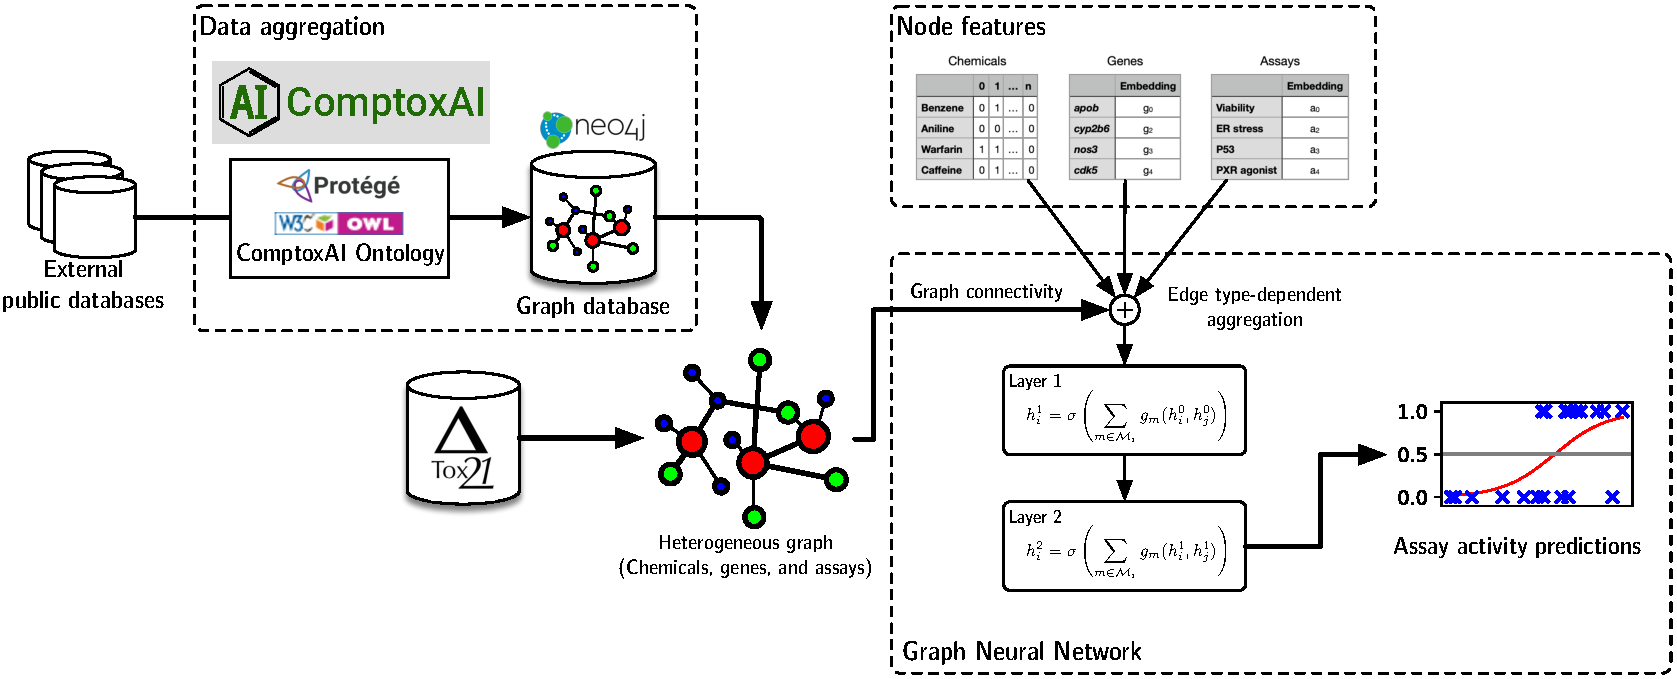
\includegraphics[width=\textwidth]{figures/figure1.pdf}
   \caption{Schematic overview of the graph machine learning approach used in this study. We build a toxicology-focused graph database (named ComptoxAI) using data aggregated from many public databases, and extract a subgraph for QSAR analysis containing chemicals, assays, and genes. We then train and evaluate a graph neural network that predicts whether or not a chemical activates specific toxicology-focused assays from the Tox21 database.}
\end{figure}

\section{Methods}

\subsection{Obtaining toxicology assay data}
We used the Tox21 dataset---which is a freely available resource produced collaboratively by the US National Institutes of Health, the US Food and Drug Administration, and the US Environmental Protection Agency---to obtain a set of candidate assays for classification and establish `ground truth' relationships between specific chemicals and those assays.
Each assay is presented along with experimental screening results describing the response of the assay to exposure to specific chemicals of toxicological interest, which includes pharmaceutical drugs, small molecule metabolites, environmental toxicants and others.
We removed all screening experiments with inconclusive or ambiguous results, as well as assays with very few (e.g., $<100$) active chemicals.

\subsection{Aggregating publicly available multimodal graph data}
The graph data used in this study come from a new data resource for computational toxicology, named ComptoxAI.
ComptoxAI includes a large graph database containing many entity and relationship types that pertain to translational mechanisms of toxicity, all of which are sourced from third-party public databases (including PubChem, Drugbank, the US EPA's Computational Toxicology Dashboard, NCBI Gene, and many others).
We extracted the subgraph from ComptoxAI's graph database defined as all nodes representing chemicals, genes, and toxicological assays, as well as the complete set of edges linking nodes of those types.
The full graph database for ComptoxAI can be found at \url{https://comptox.ai}, and will be described in a separate, upcoming publication.

\begin{figure}
   \centering
   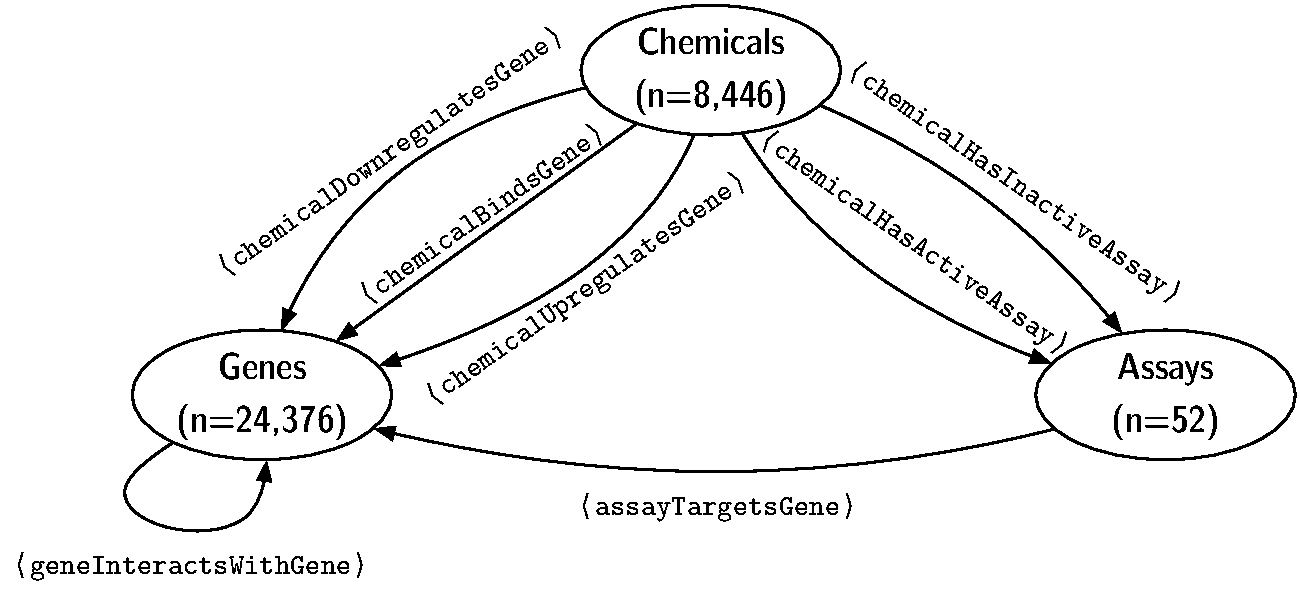
\includegraphics[width=0.7\textwidth]{figures/figure1-1.pdf}
   \caption{Metagraph describing the node types, node counts, and edge types in the heterogeneous graph. During implementation of the GNN, we also define corresponding inverse edges (e.g., assayTargetsGene $\to$ geneTargetedByAssay) to facilitate the message-passing paradigm of the GNN.}\label{fig:2}
\end{figure}

The 3 entity types that comprise the nodes of the extracted subgraph are \textit{chemicals}, \textit{assays}, and \textit{genes}.
We sourced the chemicals from the US EPA's DSSTox database, and further filtered them so that each one is equivalent to a distinct compound in PubChem.
We obtained genes from the NCBI Gene database, and assays from the Tox21 screening repository as described above.
All edges in the graph were sourced from either the Hetionet database or from assay--chemical annotations in Tox21.
A metagraph describing the node and edge types in the subgraph is shown in \textbf{Figure~\ref{fig:2}}.

\subsection{Heterogeneous graph neural network}
We constructed a heterogeneous graph convolutional neural network (GCNN) architecture for the graph ML experiments.
Since our approach uses multiple entity types (e.g., chemicals, genes, assays) in the same graph---each with possibly different sets of node features, and linked by multiple semantically distinct edge types---the architecture extends the common GCNN model to learn separate message passing functions for each edge type.
Briefly, each layer of the network aggregates signals from adjacent nodes in the graph, such that a greater number of layers results in signals being aggregated from an increasingly wider radius around each node.
The output of the network can be thought of as encoded representations of nodes that incorporate information from other nodes in their local neighborhood.
Additionally, GCNNs can be thought of as a generalization of convolutional neural networks (CNNs) used in computer vision---instead of the convolutional operator aggregating signals from nearby pixels in an image, it aggregates features from adjacent nodes in the graph.

In a heterogeneous graph, different node types represent different types of entities, each represented within a semantically distinct feature space.
Therefore, the process of aggregating information from adjacent nodes must take those nodes' types into account.
Additionally, different edge types (e.g., `chemicalUpregulatesGene' and `chemicalDownregulatesGene') convey their own semantically distinct meanings, which can substantially effect the flow of information through the network.
To handle these two challenges, we learn separate aggregation functions for each edge type in the graph, following the example proposed by Schlichtkrull \textit{et al} in R-GCNs (Relational Graph Convolutional Networks)~\cite{schlichtkrull2018modeling}.
Within the R-GCN paradigm, the aggregation process can be split into 3 sequential steps: (1.)~collecting signals from adjacent nodes using an appropriate edge type-specific message function $\phi$, (2.)~combining each of those incoming signals (across all edge types) via a reduce function $\rho$, and (3.)~finally updating the target node $v$ by applying an update function $\psi$.
Training the network is roughly equivalent to finding an appropriate parameterization of $\phi$ for each edge type.

A formal description of the GNN is given in \textbf{Appendix~\ref{GCNN}}.

% We use a message passing strategy similar to GraphSAGE~\cite{hamilton2017inductive}, where signals propagated from adjacent nodes are aggregated using their arithmetic mean:
% \begin{equation}
% \mathbf{h}_v^k \gets \sigma\left(\mathbf{W} \cdot \textsc{Mean}(\{\mathbf{h}_v^{k-1}\}\cup \{ \mathbf{h}_u^{k-1},\forall u \in \mathcal{N}(v) \})\right)
% \end{equation}
% where $\mathbf{h}_v^{k}$ is an encoded representation of the input vector $\mathbf{x}$ of node $v$ at layer $k$ of the network, $\mathbf{W}$ is a weight matrix, and $\mathcal{N}(v)$ is the neighborhood of all nodes adjacent to $v$.
% Each layer in the network `pulls' information from an increasingly wider radius around each node $v$.
% $\sigma$ is an activation applied to the output of each layer, which we define as the leaky ReLU function:
% \begin{equation}
% \sigma(x) =
% \begin{cases}
%    x & \quad \text{if } x > 0,\\
%    0.01x & \quad \text{otherwise}
% \end{cases}
% \end{equation}

\subsubsection{Node classification model}\label{methods-nc}
Our node classification task consists of labeling chemicals according to whether they do (1) or do not (0) activate a specific Tox21 assay.
The procedure we use for generating these labels is as follows:
\begin{enumerate}
   \item For each $c \in \mathcal{C}$ is adjacent to the assay of interest $a \in \mathcal{A}$, generate labels according to the following scheme:
   \begin{enumerate}
      \item 1 if there exists an edge $(c, r, a)$ such that the edge type of $r$ is \texttt{chemicalHasActiveAssay}.
      \item 0 if there exists an edge $(c, r, a)$ such that the edge type of $r$ is \texttt{chemicalHasInactiveAssay}.
      \item If both of the two preceding conditions are false, no label is generated.
   \end{enumerate}
   \item Delete $a$ (and all edges incident to $a$) from the graph.
\end{enumerate}

\begin{algorithmic}
   
\end{algorithmic}
The resulting graph $\mathcal{G}_a^\star$ is then used in a standard supervised learning task where the goal is to predict the labels on nodes corresponding to chemicals, which represent whether the assay is or is not activated in response to perturbation by that chemical.
We use an 80\%/20\% train/test split on the labeled chemicals, optimize the GCNN's parameters using the Adam algorithm (a computationally efficient variant of stochastic gradient descent suitable for sparse gradients)~\cite{kingma2014adam}, and compute the error between predicted and true labels via cross entropy loss.

To assess the contribution of the MACCS molecular descriptors when added to the GNN, we trained the node classification model both in the presence and in the absence of MACCS bitstrings applied as node features to each chemical.
Intuitively, the model trained without MACCS node features performs inference using only the graph's topological structure---including gene interactions and activity annotations to the other Tox21 assays---while the one with MACCS node features additionally has access to the same chemical structure information used in the non-graph (baseline) QSAR models.

Specific details for the node classification task are given in \textbf{Appendix~\ref{NC}}.

\subsection{Baseline QSAR classifiers}
To assess the relative performance of the GNN classification model, we built 2 additional (non-NN) QSAR models that represent well-established current practice in predictive toxicology: A random forest classifier, and a gradient boosting classifier.
Each model was trained on the aforementioned MACCS fingerprints of chemicals computed from SMILES strings, with an 80\%/20\% training/testing split.
We tuned 6 hyperparameters for each random forest model, and 5 for each gradient boosting model, as described in \textbf{Table S1}.
These were tuned using grid search, where the optimal hyperparameter set is defined as the one minimizing binary cross entropy between predicted labels and true labels on the training data.

\section{Results}
\subsection{GNN node classification performance vs.\ baseline QSAR models}
Of the 68 total assays in the Tox21 database, we retained 52 for analysis in the QSAR experiments.
The remaining 16 assays were not used due to either a low number of active chemicals or underrepresentation of screened chemicals in the ComptoxAI graph database.
As mentioned above, we discarded compounds with inconclusive or ambiguous screening results.

\begin{figure}
   \centering
   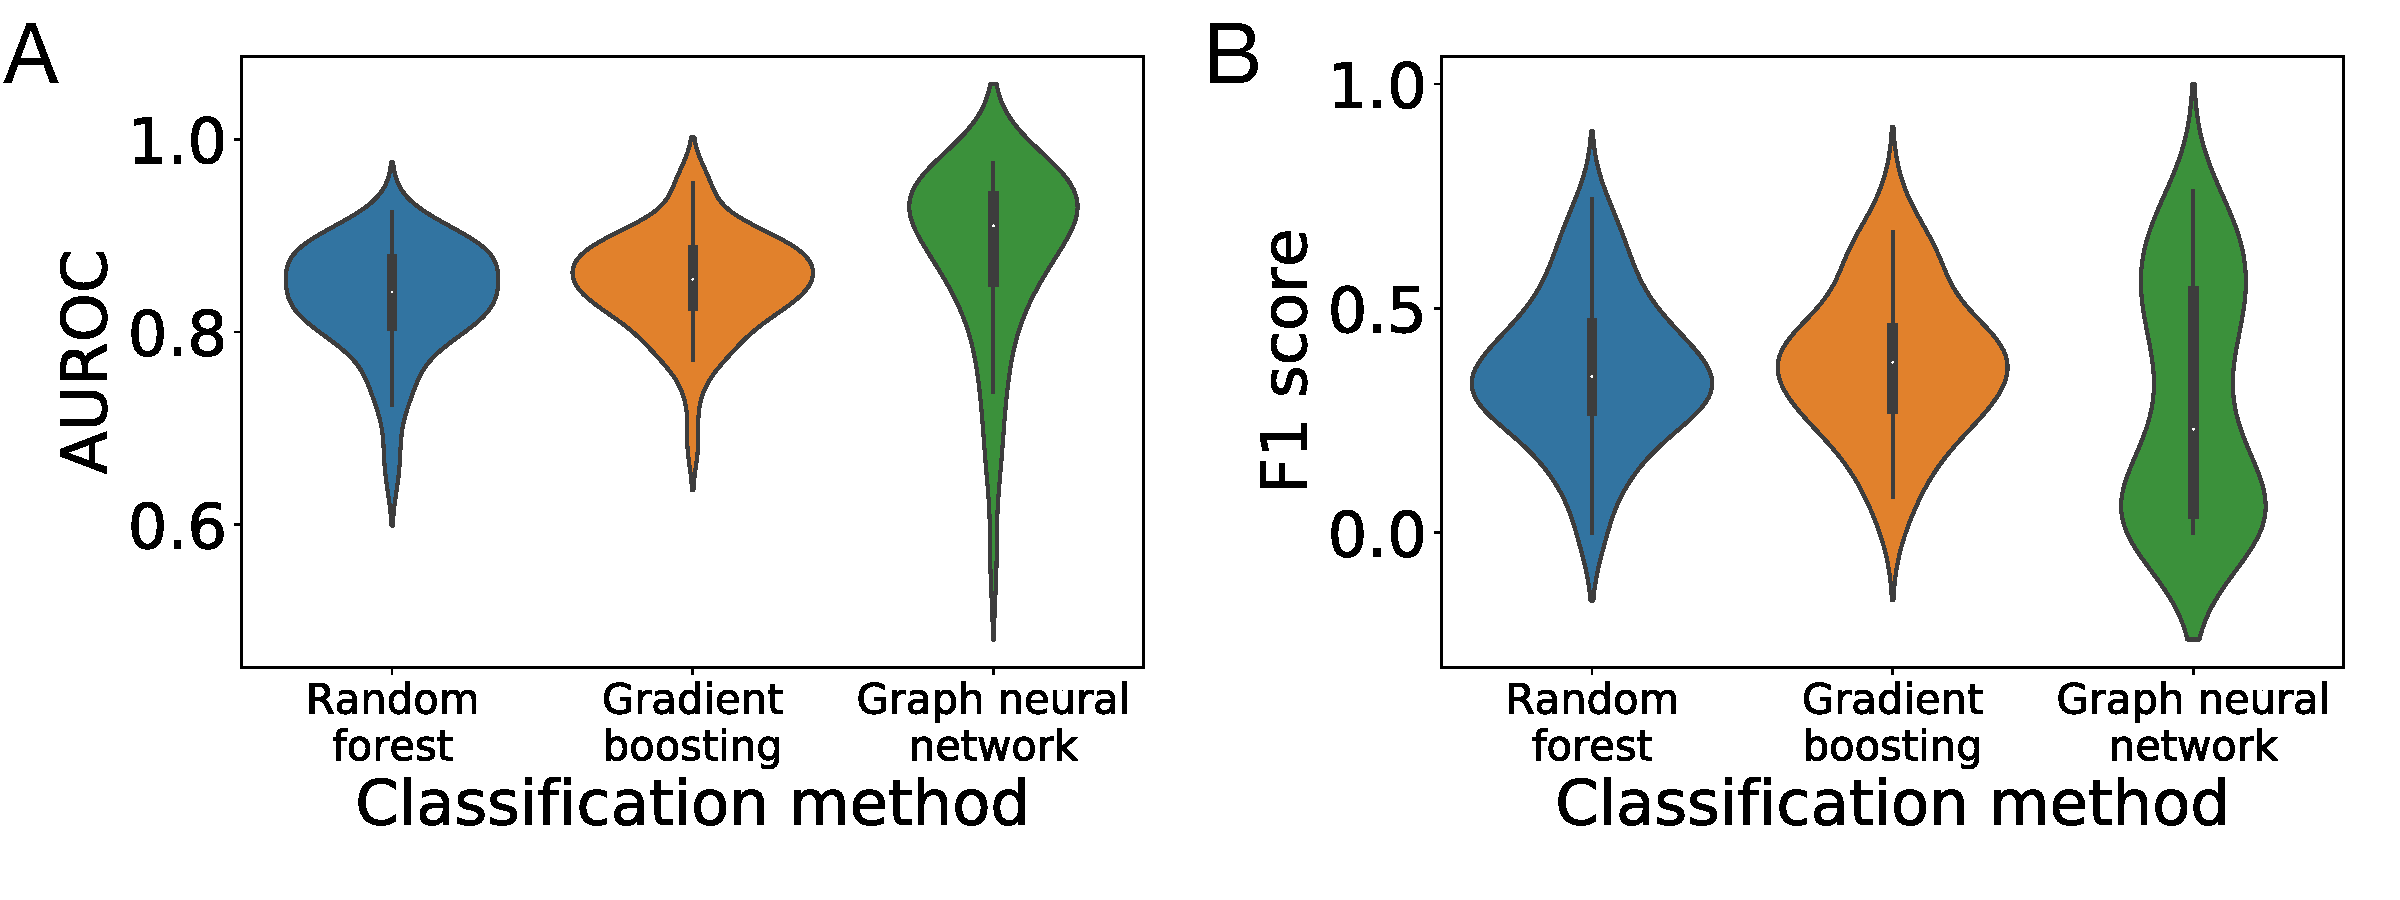
\includegraphics[width=\textwidth]{figures/figure2.pdf}
   \caption{Overall performance metrics of the 3 QSAR model types on each of the Tox21 assays---a.)~Area Under the Receiver Operator Characteristic curve (AUROC) and b.)~F1 score. The mean AUROC is significantly higher for the GNN model than for either of the two baseline QSAR approaches. The differences in F1 scores are not statistically significant. The GNN achieves poor F1 scores on assays with relatively few (e.g., $< 100$) ``active'' annotations in Tox21, which is consistent with known performance of neural networks on data with sparse labels.}\label{fig:3}
\end{figure}

\begin{figure}
   \centering
   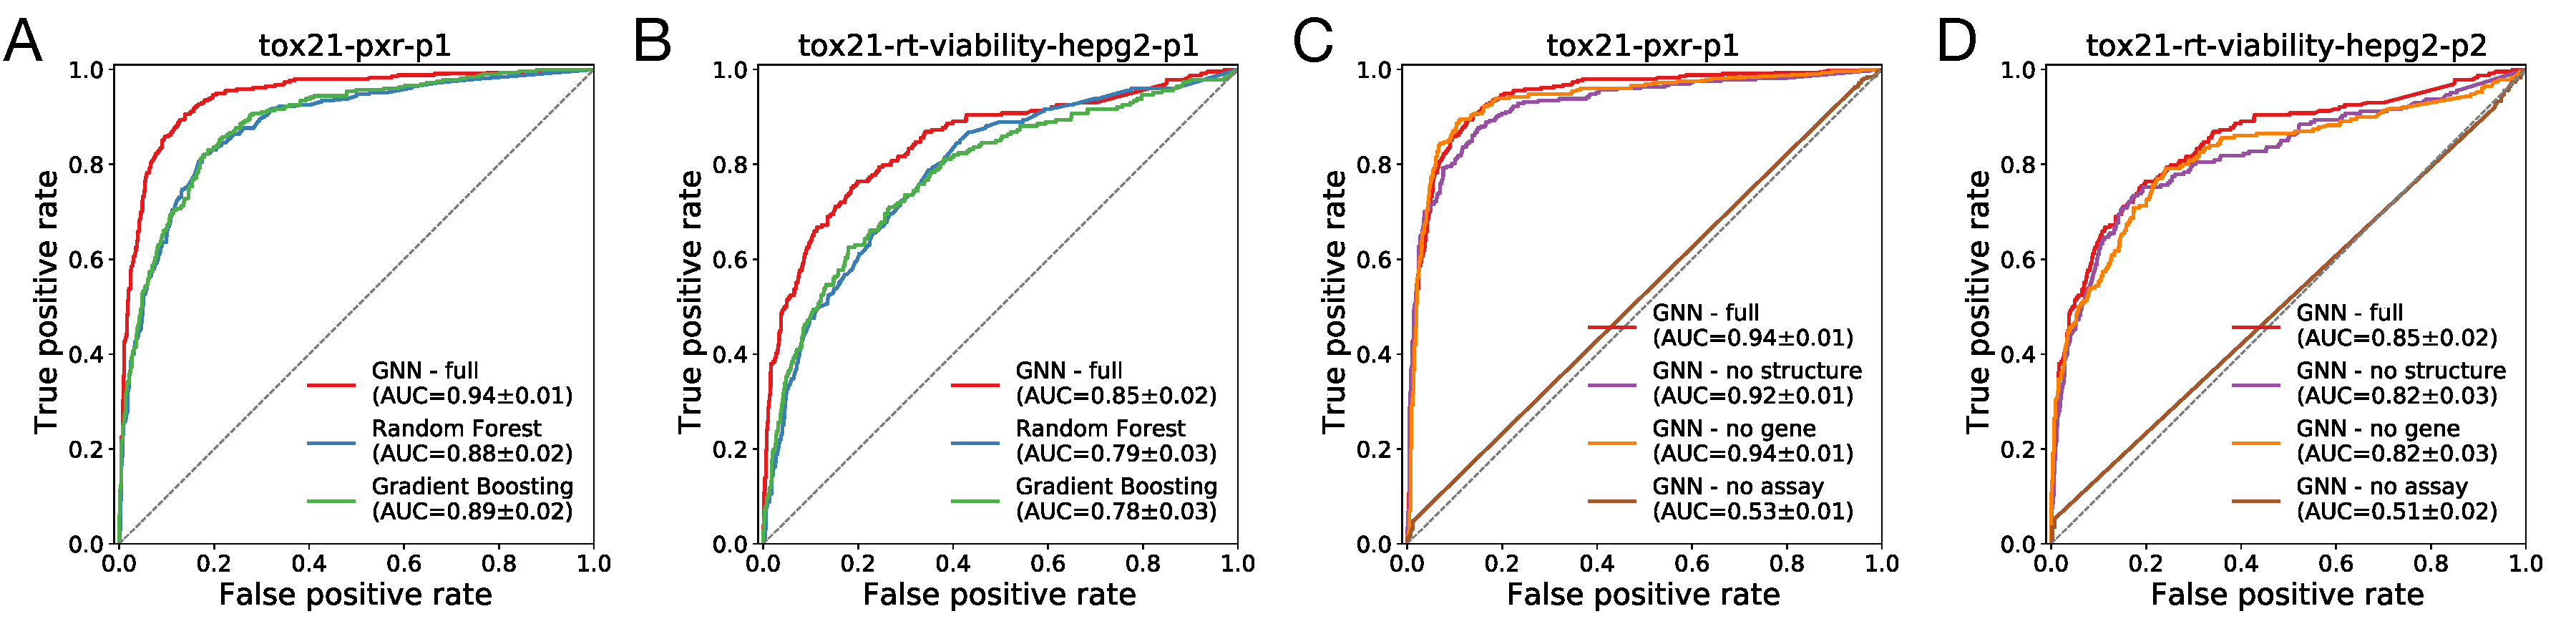
\includegraphics[width=\textwidth]{figures/figure3.pdf}
   \caption{Receiver Operator Characteristic (ROC) curves for two selected Tox21 assays: a.)~PXR agonism (\texttt{tox21-pxr-p1}) and b.)~HepG2 cell viability (\texttt{tox21-rt-viability-hepg2-p1}). In both cases, the area under the curve (AUC) is significantly higher for the GNN model than either the Random Forest or Gradient Boosting models.}\label{fig:4}
\end{figure}

\subsection{Ablation analysis of graph components' influence on the trained predictive model}

\begin{figure}
   \centering
   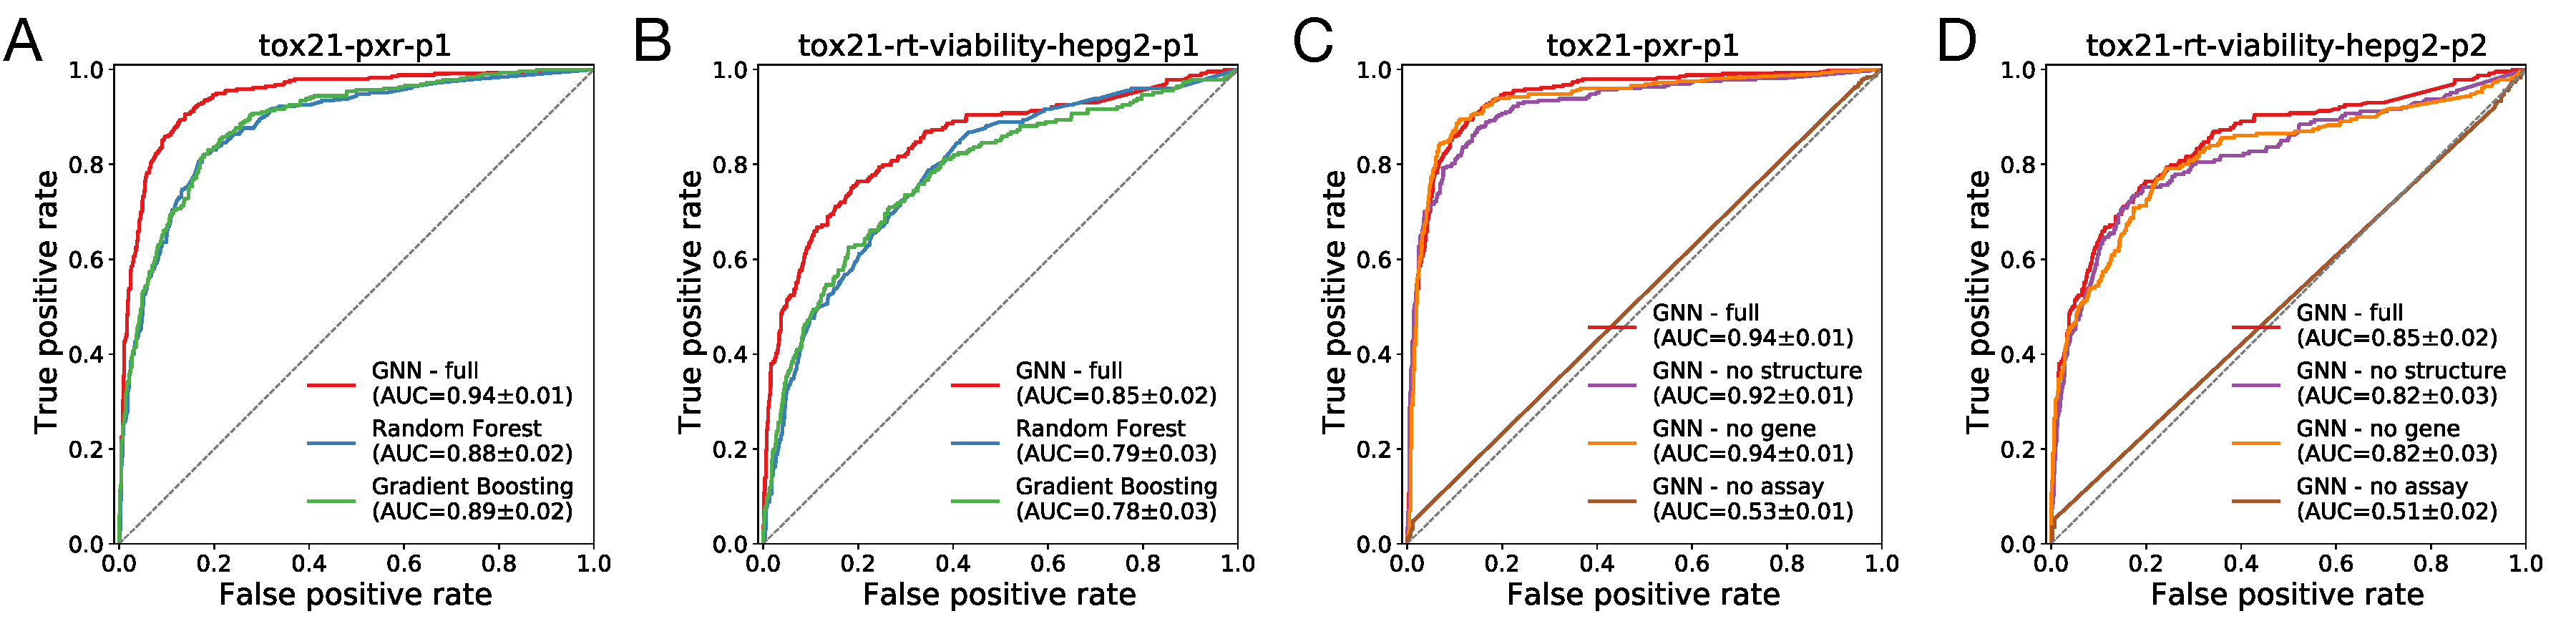
\includegraphics[width=\textwidth]{figures/figure3.pdf}
   \caption{Receiver Operator Characteristic (ROC) curves for two selected Tox21 assays using different configurations of the GNN model. `GNN - full' is the complete model as described in \S\ref{methods-nc}. `GNN - no structure' omits the MACCS chemical descriptors and replaces them with node embeddings of the same dimensionality. `GNN - no gene' removes gene nodes and their incident edges from the network. `GNN - no assay' removes all assay nodes and incident edges, so predictions are made solely using chemicals, genes, the remaining edges, and the MACCS chemical descriptors as chemical node features.}\label{fig:5}
\end{figure}

\section{Discussion}

\subsection{GNNs versus traditional ML for QSAR modeling}
The toxicology community largely agrees that QSAR underperforms on many tasks, and that new methodological advances are desperately needed.
In this study, we demonstrate that GNNs significantly outperform the current gold-standard techniques in the field.
Aside from the fact that neural networks can more easily adapt to nonlinear objectives than non-neural network models, this is likely a natural consequence of incorporating biomedical knowledge that goes beyond chemical structure characteristics.
Gene interactions provide clues about how chemicals influence metabolic and signaling pathways \textit{in vivo}, and non-target assays (i.e., other assays in the graph aside from the one currently being predicted) may correlate with activity of the target assay.

\subsection{Interpretability of GNNs in QSAR}

\subsection{Future opportunities}

\section{Conclusions}

\section{Code availability}
All source code pertaining to this study is available on GitHub at \url{https://github.com/EpistasisLab/qsar-gnn}.
A frozen copy of the code at the time of writing is available at [XXX; Zenodo].

\section{Supplemental Materials}
Supplemental tables and figures are available on FigShare at [XXX].

\section*{Acknowledgements}
This work was made possible with support from US National Institutes of Health grants \texttt{R01-LM010098}, \texttt{R01-LM012601}, \texttt{R01-AI116794}, \texttt{UL1-TR001878}, \texttt{UC4-DK112217} (PI: Jason~Moore), \texttt{T32-ES019851}, and \texttt{P30-ES013508} (PI: Trevor~Penning).

\appendix{Graph convolutional network architecture}\label{GCNN}
Some stuff here.

\appendix{Node classification model}\label{NC}
Some more stuff.

\bibliographystyle{ws-procs11x85}
\bibliography{psb-gnn}

\end{document} 

%%% \renewcommand\bibname{References\\ {\normalfont\it References can be typed in your preferred bibliography style.}}